\documentclass{standalone}

\usepackage{tikz}
\usepackage{standalone}
\usetikzlibrary{calc}
\usepackage{color}

\usetikzlibrary{decorations.pathmorphing}
\usetikzlibrary{fit}					% fitting shapes to coordinates
\usetikzlibrary{backgrounds}	% drawing the background after the foreground

\tikzstyle{background}=[red, rectangle, draw, inner sep=0.1mm,
		   rounded corners=3mm]



\begin{document}

    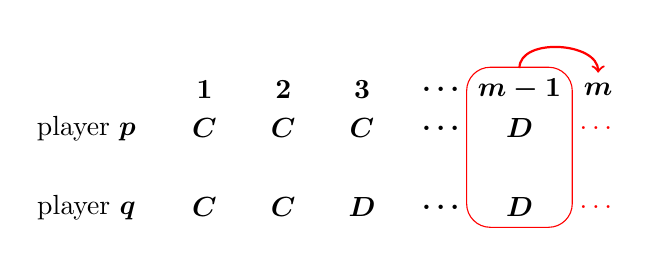
\begin{tikzpicture}

    \tikzstyle{state}=[minimum width=1cm, font=\boldmath];
    

	\node[thick] (0) at (-0.5, 0) [state] {player $p$};
	\node[thick] (1) at (-0.5, -1) [state] {player $q$};

	\node[thick] (2) at (1, 0.5) [state] {$1$};
	\node[thick] (3) at (2, 0.5) [state] {$2$};
	\node[thick] (4) at (3, 0.5) [state] {$3$};
	\node[thick] (5) at (4, 0.5) [state] {$\dots$};
	\node[thick] (6) at (5, 0.5) [state] {$m - 1$};
	\node[thick] (7) at (6, 0.5) [state] {$m$};

	\node (8) at (1, 0) [state] {$C$};
	\node (9) at (2, 0) [state] {$C$};
	\node (10) at (3, 0) [state] {$C$};
	\node (11) at (4, 0) [state] {$\dots$};
	\node (12) at (5, 0) [state] {$D$};
	\node (13) at (6, 0) [state] {\textcolor{red}\dots};

	\node (14) at (1, -1) [state] {$C$};
	\node (15) at (2, -1) [state] {$C$};
	\node (16) at (3, -1) [state] {$D$};
	\node (17) at (4, -1) [state] {$\dots$};
	\node (18) at (5, -1) [state] {$D$};
	\node (19) at (6, -1) [state] {\textcolor{red}\dots};

	\draw (6) edge[red, out=90, in=90, ->, thick] node [above] {} (7);

	\node [background, fit=(6) (12) (18)] {};

    \end{tikzpicture}

\end{document}